Overview of this part.

\chapter{Memory Object Models, explained}
\label{chap:mem-model-explained}

Explain the connection to Core -- not that strong, thanks to the memory
interface and the invariants of the VIP heaps, separation logic heaps, and
memory actions.

Factorising the formalisation pays off here.

\chapter{Pointers: more than you wanted to know}

Explain pointers in excrutiating detail, and why we need provenance for
optimisations.

Why do we care about provenance, why are pointers not just addresses

Common-subexpression elimination, copy-propogation, etc.

\section{Explaining PNVI-ae-udi and VIP}

\section{Design Space}

Alternatives

\begin{figure}[h]
    \centering
    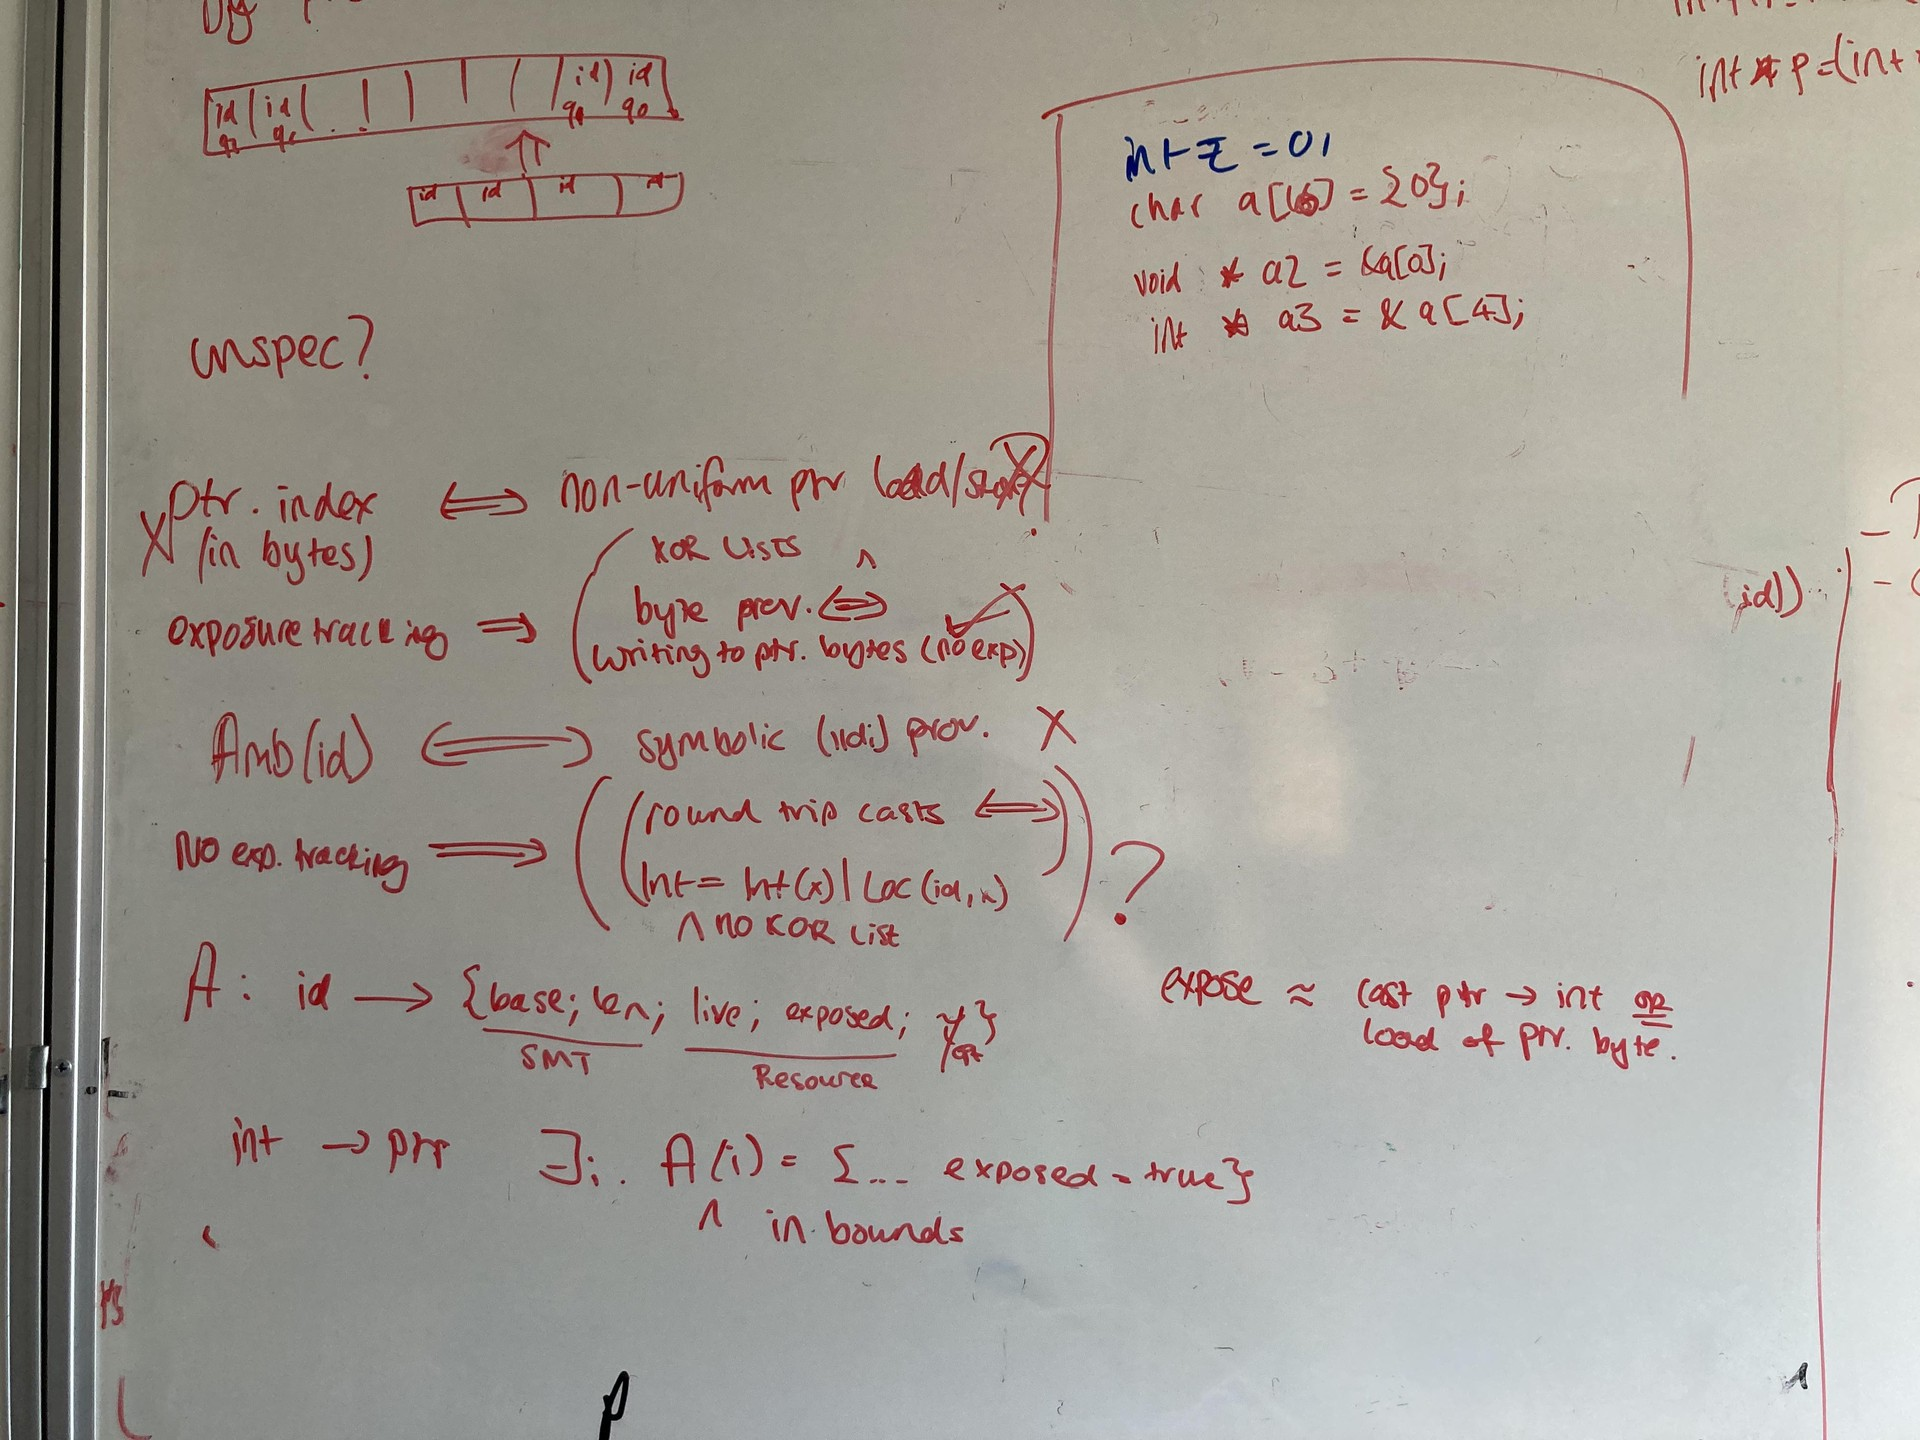
\includegraphics[width=\textwidth]{../misc/type-system-options.jpg}
\end{figure}


\section{Implementation}

Performance graph

\begin{figure}[h]
    \centering
    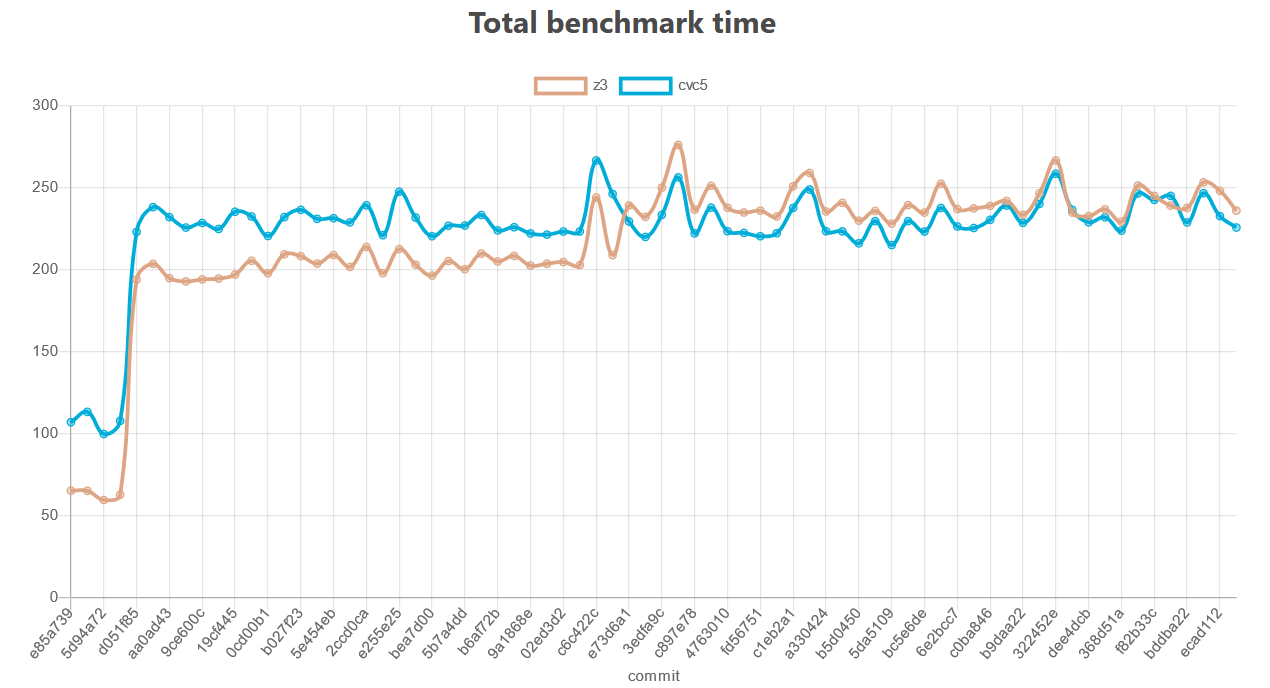
\includegraphics[width=\textwidth]{../misc/vip-performance-hit.png}
\end{figure}

\url{https://rems-project.githb.io/cerberus/dev/bench/}

\begin{comment}

\kl{Coq} is a very complex tool. Even its \kl{kernel}, which is only but a very small
fraction of it, is already quite complex: it relies on subtle implicit invariants, which
might not be properly maintained, especially when the code evolves.
In practice, around one critical bug is found every year.%
\sidenote{A \href{https://github.com/coq/coq/blob/master/dev/doc/critical-bugs}{compilation}
  of those is maintained by \kl{Coq}’s development team.}
Although it is in practice generally difficult to exploit these
and actually derive an inconsistency,
even less so inadvertently, simply relying on the \kl{De Bruijn criterion}%
\sidenote{Keeping a small, trusted kernel that is the only one responsible for the validity
of proofs.}
is not enough if one wants to trust \kl{Coq}.
Indeed, while \kl{CIC} is well-understood and has been widely studied,
this is much less true of the type theory actually implemented, \kl{PCUIC}.
Bugs therefore often creep in with the extra level of complexity coming with the implementation,
rather than being the consequence of a defect of pen-and-paper proofs.%
\sidenote{This is for instance the case of the completeness issue
  exposed in \cref{sec:bidir-pcuic-inductives}.}

These difficulties beg for a precise investigation of \kl{PCUIC}, from the heights of the
type system’s meta-theory, all the way down to the sophisticated details of the implementation.
Due to the complexity of the endeavour, it is not feasible on paper. Nor is it
desirable: if in the end we wish to implement a certified kernel, it is natural to do so
in a proof assistant, so that we can run that certified implementation.
The natural framework is thus the \kl{MetaCoq} project,
which aims at giving tools to reify and manipulate \kl{Coq} terms%
\sidenote{Or, maybe more accurately, \kl{Gallina}.}
inside \kl{Coq} itself. This gives the possibility to write down and certify
all kinds of procedures operating on these terms, the first to come to mind being of course
a type-checker. This way, we can have both the help and guarantees offered by
formal proofs inside a \kl{proof assistant}, and the possibility to execute
our implemented kernel.

There are two important caveats to this, though.
The first pertains to Gödel’s second incompleteness
theorem. Because of it, it is impossible to prove \kl{Coq}’s consistency
inside \kl{Coq} itself,
meaning that the meta-theoretical study can only be partial, since otherwise it would allow
a proof of consistency contradicting Gödel’s theorem. In
\kl{MetaCoq}, this blind spot manifests as an axiom assuming the
\kl{normalization} of \kl{PCUIC}, on which parts of the development relies.
The second caveat is that writing down a certified kernel is not enough.
Indeed, executing directly such a kernel in \kl{Coq}
would be much too slow to actually type-check any reasonably-sized term.
Rather, we must rely on extraction, a procedure which erases the
proof-related content of a certified program to only keep the algorithmically relevant one.
As this erasure itself is a complex transformation, \kl{MetaCoq} also incorporates a certified
erasure procedure.

In this part of the thesis,
I shall describe the portion of \kl{MetaCoq} which is relevant to it.
\Cref{chap:metacoq-general} gives a general overview of
the meta-theory of \kl{PCUIC}, with the main definitions, properties, and proof ideas.
My technical contributions to this part of the development is relatively minor,
mainly consisting of small patches. However, since I rely on that formalization
in my main contributions, it seems fitting to go over it.

\Cref{chap:kernel-correctness} concentrates on the formalization of bidirectional typing, as
presented in \arefpart{bidir}, and on the proof of correctness and completeness of
the kernel implementation based on it. This is my main technical
contributions to the \kl{MetaCoq} project.

Although I will not describe it here, there is more to \kl{MetaCoq}. The two main components
I will omit are Template \kl{Coq}, and the certified extraction procedure.
The first faithfully represents the actual abstract
syntax tree of \kl{Gallina} and a typing predicate for it,
gives a translation to the syntax used in the main theoretical development of \kl{PCUIC},%
\sidenote{Described in \cref{fig:metacoq-ast}.}
and shows that both notions of typing are equivalent.
It also provides facilities for quoting and unquoting of terms from
\kl{Coq} to \kl{MetaCoq}’s AST and back, in order to provide the possibility to write operation
on \kl{Coq} terms directly in \kl{MetaCoq} – including, of course, the certified kernel of
\cref{chap:kernel-correctness}.
The second component aims at certifyng the extraction procedure,
relating the semantics of the original and extracted programs.
The goal is to be able to extract the certified type-checker itself to an efficient one –
execution in \kl{Coq} is too inefficient if we wish to type-check realistic examples –,
but also more generally to improve \kl{Coq}’s current extraction.

Throughout the part, source files of the \kl{MetaCoq} project
and specific definitions or theorems are referenced respectively as follows:
\pcuicfile{Typing}, and \pcuicline{Typing}{typing}{188}. They link directly to the source
code of the project on \kl{GitHub} – on a branch dedicated to this thesis.

\end{comment}
